%%%%%%%%%%%%%%%%%%%%%%%%%%%%%%%%%%%%%
% Stylish Article
% LaTeX Template
% Version 2.0 (13/4/14)
%
% This template has been downloaded from:
% http://www.LaTeXTemplates.com
%
% Original author:
% Mathias Legrand (legrand.mathias@gmail.com)
%
% License:
% CC BY-NC-SA 3.0 (http://creativecommons.org/licenses/by-nc-sa/3.0/)
%
%%%%%%%%%%%%%%%%%%%%%%%%%%%%%%%%%%%%%%%%%

%----------------------------------------------------------------------------------------
%	PACKAGES AND OTHER DOCUMENT CONFIGURATIONS
%----------------------------------------------------------------------------------------

\documentclass[fleqn,10pt]{SelfArx} % Document font size and equations flushed left



%----------------------------------------------------------------------------------------
%	COLUMNS
%----------------------------------------------------------------------------------------

\setlength{\columnsep}{0.55cm} % Distance between the two columns of text
\setlength{\fboxrule}{0.75pt} % Width of the border around the abstract

%----------------------------------------------------------------------------------------
%	COLORS
%----------------------------------------------------------------------------------------

\definecolor{color1}{RGB}{0,0,90} % Color of the article title and sections
\definecolor{color2}{RGB}{0,20,20} % Color of the boxes behind the abstract and headings

%----------------------------------------------------------------------------------------
%	HYPERLINKS
%----------------------------------------------------------------------------------------

\usepackage{hyperref} % Required for hyperlinks
\hypersetup{hidelinks,colorlinks,breaklinks=true,urlcolor=color2,citecolor=color1,linkcolor=color1,bookmarksopen=false,pdftitle={Title},pdfauthor={Author}}

%----------------------------------------------------------------------------------------
%	ARTICLE INFORMATION
%----------------------------------------------------------------------------------------

\JournalInfo{Taller de Biotecnología Animal, 2014-I} % Journal information
\Archive{Review} % Additional notes (e.g. copyright, DOI, review/research article)

\PaperTitle{Transfección en Animales} % Article title

\Authors{Juan Manuel Iglesias Artola\textsuperscript{1}, Gianfranco Villamonte Cuneo\textsuperscript{1}} % Authors
\affiliation{\textsuperscript{1}\textit{School of Biology, Universidad Ricardo Palma, Lima, Peru}} % Author affiliation
%\affiliation{\textsuperscript{2}\textit{Department of Chemistry, University of Examples, London, United Kingdom}} % Author affiliation
\affiliation{*\textbf{Corresponding authors}: jmanuel9112@icloud.com / giancuneo@gmail.com } % Corresponding author


%----------------------------------------------------------------------------------------
%	ABSTRACT
%----------------------------------------------------------------------------------------

\Abstract{}


\Keywords{Keyword1 --- Keyword2 --- Keyword3} % Keywords - if you don't want any simply remove all the text between the curly brackets
\newcommand{\keywordname}{Palabras clave} % Defines the keywords heading name

%----------------------------------------------------------------------------------------

\begin{document}

\flushbottom % Makes all text pages the same height

\maketitle % Print the title and abstract box

\tableofcontents % Print the contents section

\thispagestyle{empty} % Removes page numbering from the first page

%----------------------------------------------------------------------------------------
%	ARTICLE CONTENTS
%----------------------------------------------------------------------------------------

\section{Introducción} 

\addcontentsline{toc}{section}{Introducción} % Adds this section to the table of contents


 and some mathematics $\cos\pi=-1$ and $\alpha$ in the text\footnote{And some mathematics $\cos\pi=-1$ and $\alpha$ in the text.}.

%------------------------------------------------

\section{Métodos de Transfección}

\begin{figure*}[ht]\centering % Using \begin{figure*} makes the figure take up the entire width of the page
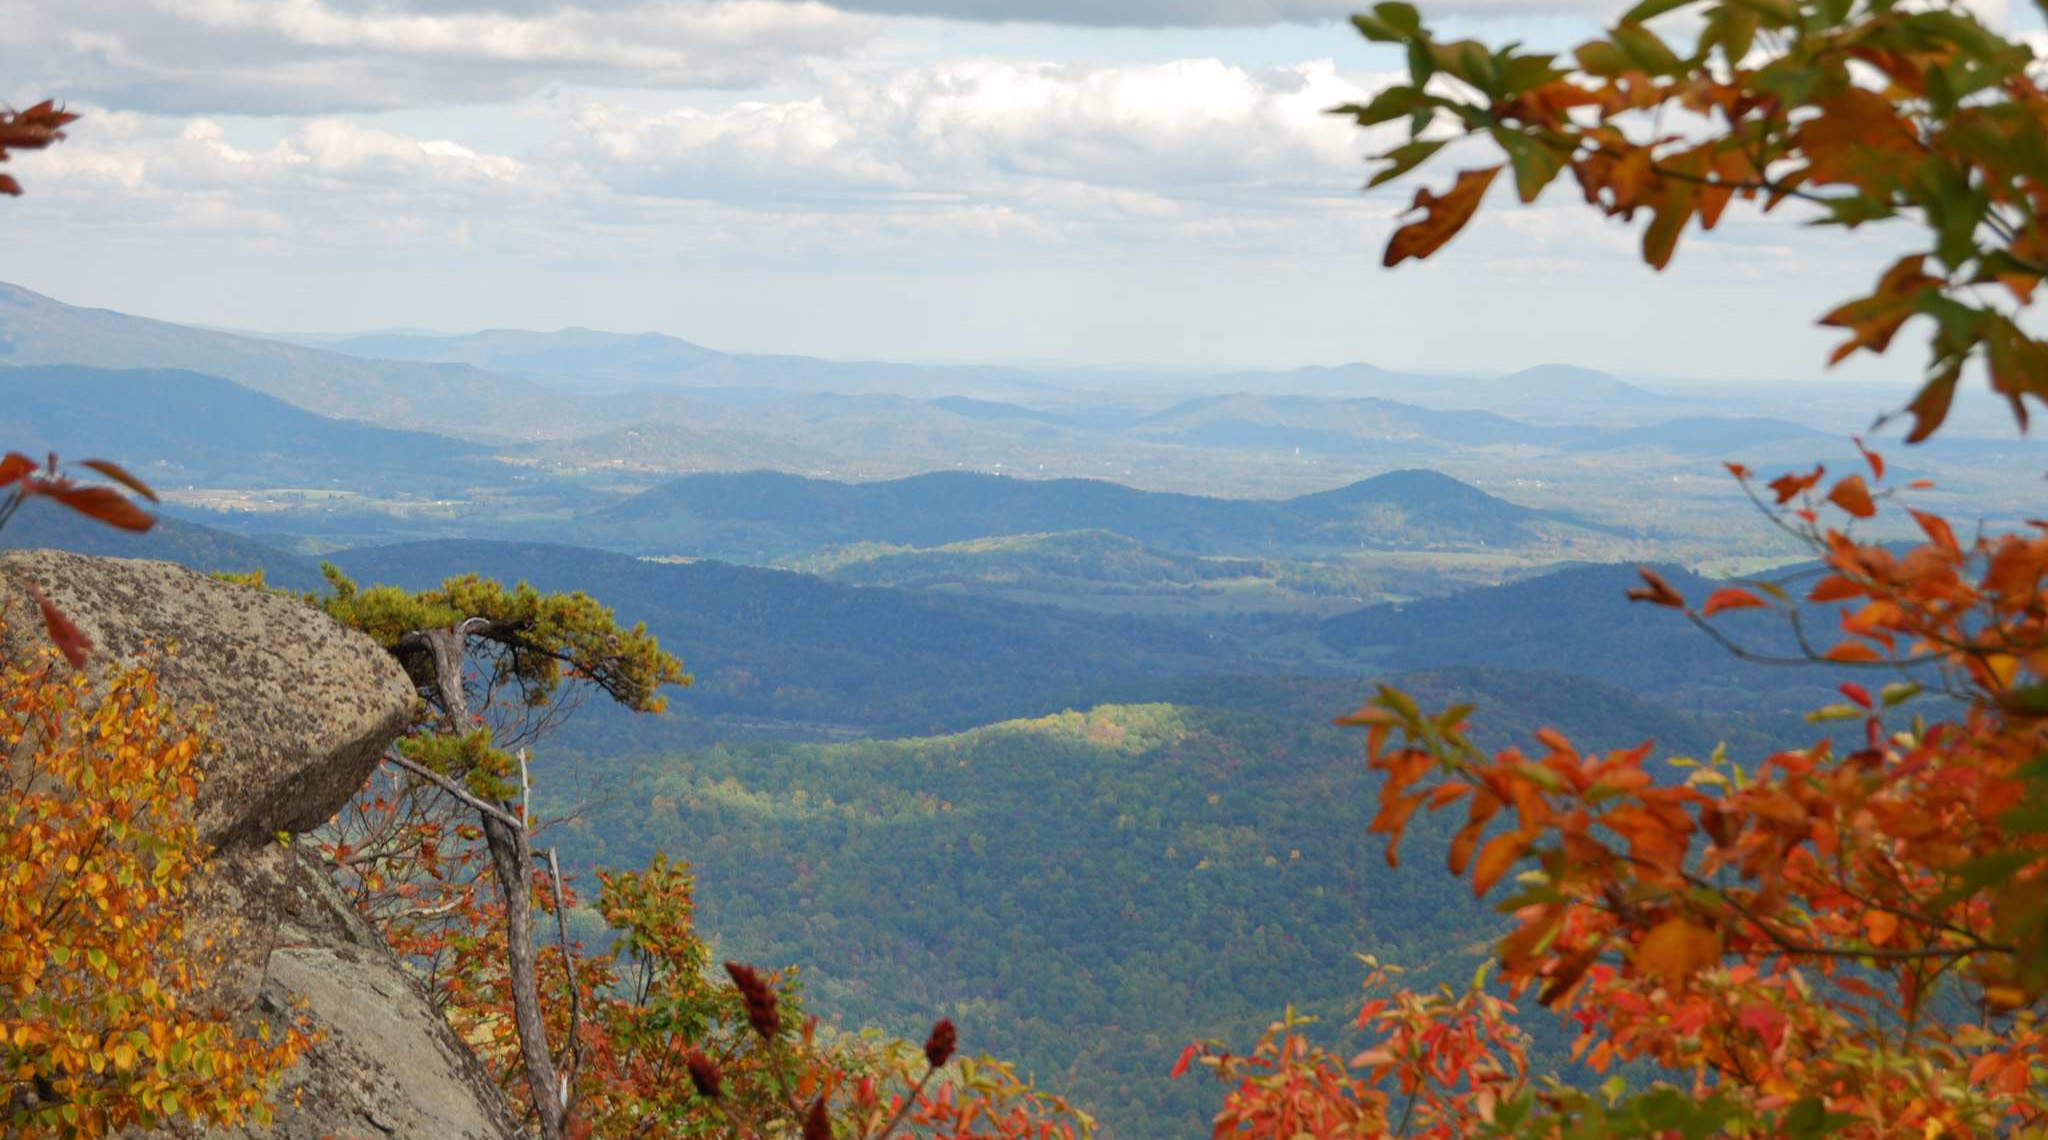
\includegraphics[width=\linewidth]{images/view}
\caption{Wide Picture}
\label{fig:view}
\end{figure*}


\begin{equation}
\cos^3 \theta =\frac{1}{4}\cos\theta+\frac{3}{4}\cos 3\theta
\label{eq:refname2}
\end{equation}



\begin{enumerate}[noitemsep] % [noitemsep] removes whitespace between the items for a compact look
\item First item in a list
\item Second item in a list
\item Third item in a list
\end{enumerate}

\subsection{Subsection}



\paragraph{Paragraph} %\lipsum[7] % Dummy text
\paragraph{Paragraph} %\lipsum[8] % Dummy text

\subsection{Subsection}



\begin{figure}[ht]\centering
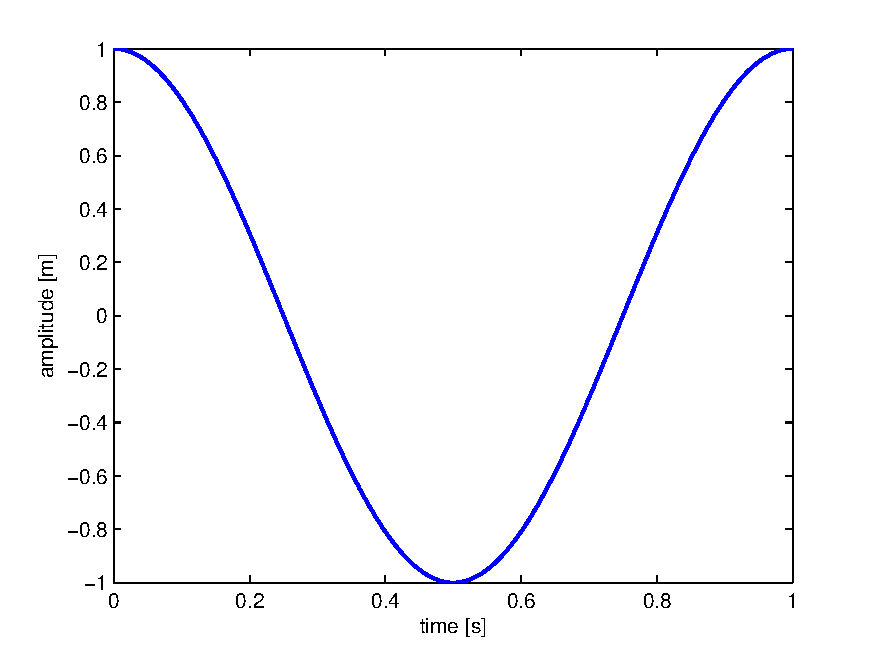
\includegraphics[width=\linewidth]{images/results}
\caption{In-text Picture}
\label{fig:results}
\end{figure}

Reference to Figure \ref{fig:results}.

%------------------------------------------------

\section{Aplicaciones de la Transfección}

La transfección es una herramienta para la modificación genética. Gracias a sus múltiples métodos es posible realizar innumerables aplicaciones como:
\begin{itemize}[noitemsep] % [noitemsep] removes whitespace between the items for a compact look
\item \textbf{Terapia Génica}: Cura de enfermedades.
\item \textbf{Animales Transgénicos}: Mejoramiento para alimentación.
\item \textbf{Estudios Genéticos}: Genes 'knockout' o 'knockdown' para estudiar su expresión fenotípica.
\item \textbf{Fábricas Vivientes}: Producción de proteínas recombinantes utilizando animales.
\end{itemize}


\subsection{\textbf{Terapia Génica}}

%\lipsum[11] % Dummy text

\begin{table}[hbt]
\caption{Table of Grades}
\centering
\begin{tabular}{llr}
\toprule
\multicolumn{2}{c}{Name} \\
\cmidrule(r){1-2}
First name & Last Name & Grade \\
\midrule
John & Doe & $7.5$ \\
Richard & Miles & $2$ \\
\bottomrule
\end{tabular}
\label{tab:label}
\end{table}

\subsection{Animales Transgénicos}

%\lipsum[12] % Dummy text

\begin{description}
\item[Word] Definition
\item[Concept] Explanation
\item[Idea] Text
\end{description}

\subsection{Estudios Genéticos}

%\lipsum[13] % Dummy text

\begin{itemize}[noitemsep] % [noitemsep] removes whitespace between the items for a compact look
\item First item in a list
\item Second item in a list
\item Third item in a list
\end{itemize}

\subsection{Fábricas Vivientes}

%\lipsum[14] % Dummy text

\subsection{Subsection}

%\lipsum[15-23] % Dummy text

%------------------------------------------------

\section{Implicancias Bioéticas de la Transfección}

%\lipsum[10] % Dummy text

%------------------------------------------------
\phantomsection
\section*{Acknowledgments} % The \section*{} command stops section numbering

\addcontentsline{toc}{section}{Acknowledgments} % Adds this section to the table of contents

So long and thanks for all the fish \cite{khaliligene2006}.

%----------------------------------------------------------------------------------------
%	REFERENCE LIST
%----------------------------------------------------------------------------------------

\newpage
\section*{Referencias Bibliográficas}
\addcontentsline{toc}{section}{Referencias Bibliográficas}
\bibliographystyle{unsrt}
\bibliography{referencias}

%----------------------------------------------------------------------------------------

\end{document}
